
% \begin{table}[t]

% % \caption{\small \emph{Left:} The sequence error for SVHN multi-digit recognition
% % on crops of $64\times 64$ pixels (64px), and inflated crops of $128 \times 128$
% % (128px) which include more background. \textsuperscript{*}The best reported
% % result from \cite{Ba14} uses model averagin}
% % % }}%
% \vspace{-1em}
% \end{table}


\begin{table}[t]
\begin{center}\small
% \setlength{\tabcolsep}{3pt}
    \begin{tabular}{lc}
        \toprule
        \multicolumn{1}{c}{Method}& mean IOU  \\
        \midrule
        % DenseASPP \cite{Yang2018DenseASPP}&  80.6 \\
        % SPG  \cite{Cheng2019SPGNet}  &     $81.1$        \\
        % DANet  \cite{Fu2018DANet} &     $81.5$        \\
        HRNetv2  \cite{Sun2019HRNet}     &     $81.8$        \\
        EMANet  \cite{Li2019EMANet}&     $81.9$        \\
        ACNet \cite{Fu2019ACNet}&  \secbest{82.3}        \\
        \midrule
        Our Baseline  &     80.9        \\
        Ours WRP + UAT  &     \best{82.3}        \\
        \bottomrule
    \end{tabular}
\qquad\qquad \qquad\qquad
% \hspace{-2em}
% \vtop{
% \vspace{-1em}
% \hbox{
% 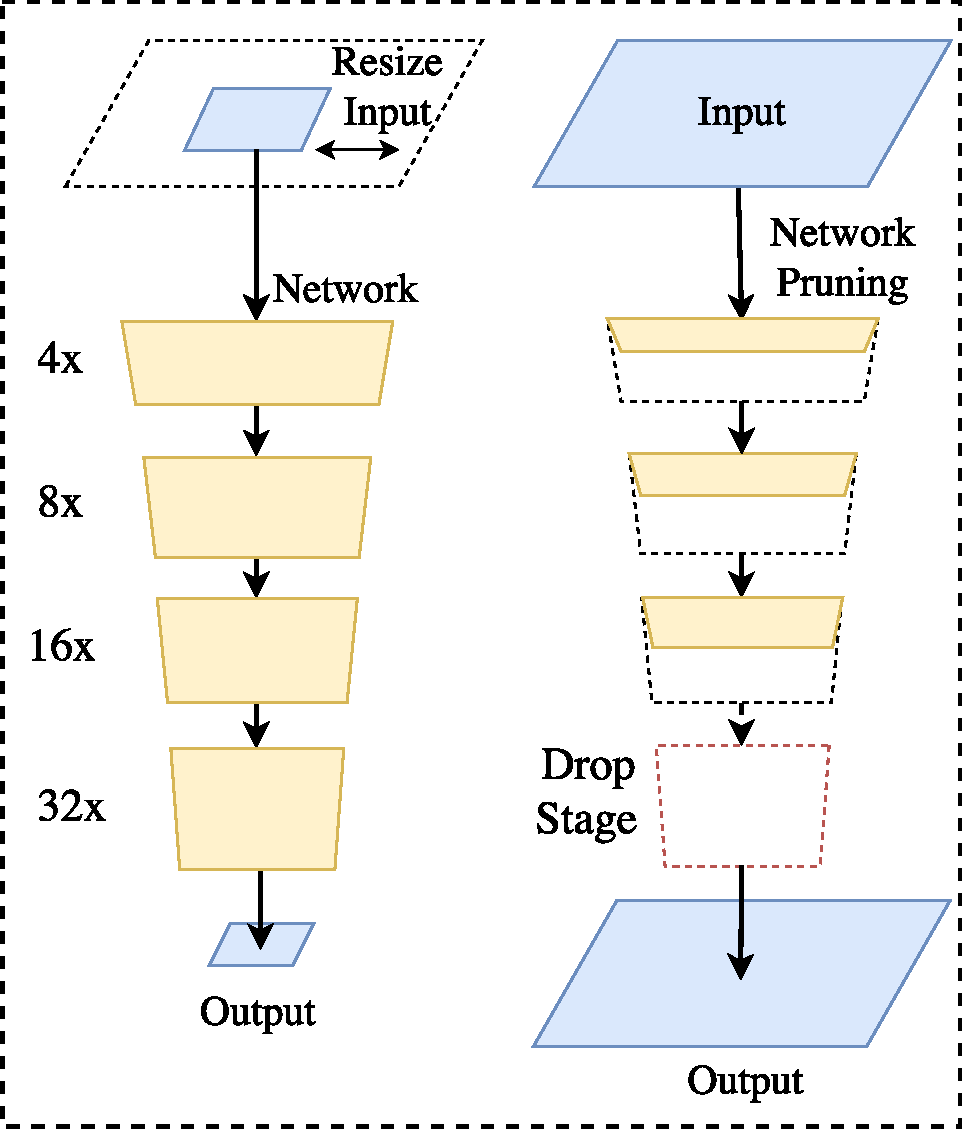
\includegraphics[width=0.6\textwidth]{figures/input_model.pdf}
    \begin{tabular}{llcc}
        \toprule
        \multicolumn{2}{c}{Dataset}& Loss & mean IOU  \\
        \midrule
        \multicolumn{2}{l}{$D_L$} & C.E. & 77.62\\
        \multicolumn{2}{l}{$D_L$ + \cite{nvidia_cvpr19} ($\pm 2,4,6,8$)}& RLL &77.82  \\
        \multicolumn{2}{l}{$D_L$ + Ours ($\pm [2,4,6,8])$}&$\mathtt{UAT}$ & 78.45  \\
        \midrule
        \multicolumn{2}{l}{$D_L$ + GT($\pm [2,4,6,8])$}& \cite{gal_main} & 77.82  \\
        \bottomrule
    \end{tabular}

% }}%
\end{center}
\caption{\small \emph{Left:} The sequence error for SVHN multi-digit recognition
on crops of $64\times 64$ pixels (64px), and inflated crops of $128 \times 128$
(128px) which include more background. \textsuperscript{*}The best reported
result from \cite{Ba14} uses model averagin}
\label{table:svhn}
\end{table}
